\textbf{\underline{OZ 4 - De wet van Ampère en de wet van Biot-Savart - Oefening 5:}}
\vspace{0.5cm}

% \begin{minipage}{0.64\textwidth}
%     Een lange cilindrische geleider met straal $a$ heeft twee cilindrische gaten van diameter $a$ doorheen zijn hele lengte (zie doorsnede in Figuur 5). Een stroom $I$ vloeit door de geleider en is uit het blad gericht. De stroomdichtheid is uniform doorheen de doorsnede van de draad. Wat is het magnetisch veld in termen van $\mu_0$, $I$, $r$ en $a$ in punt $P_1$? Dezelfde vraag voor punt $P_2$.
%     \vspace{1cm}
% \end{minipage}
% \begin{minipage}{0.32\textwidth}
%     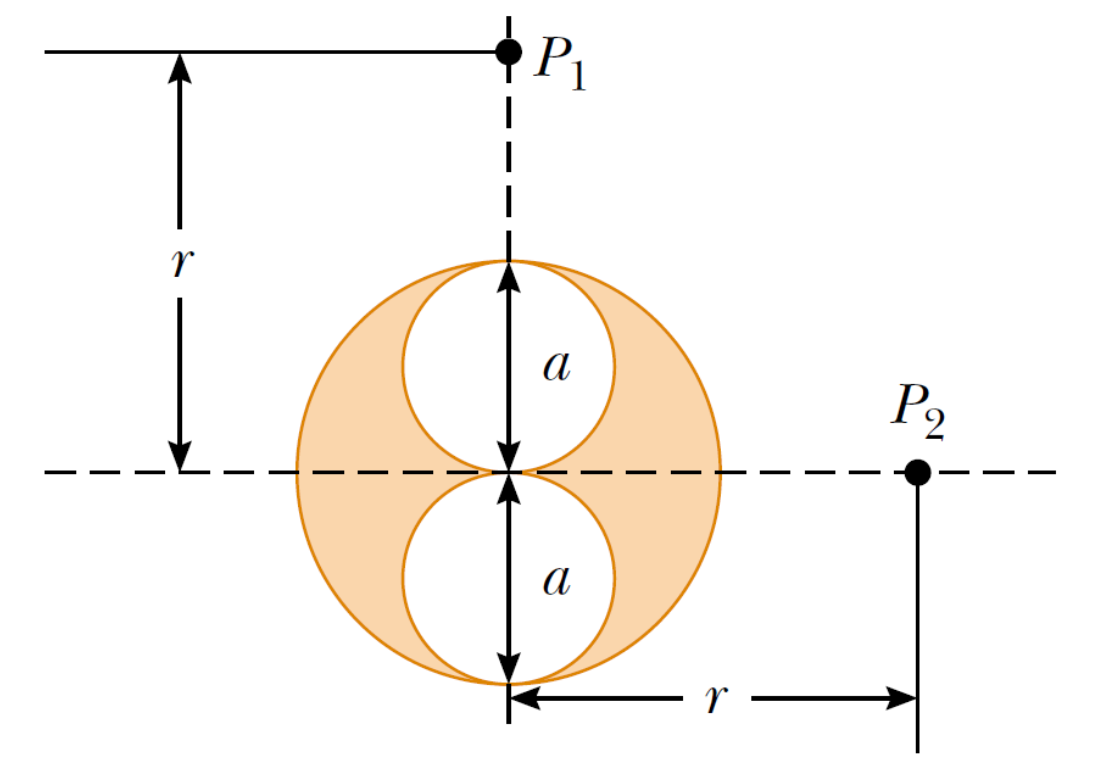
\includegraphics[scale = 0.25]{oz04/resources/Oz4Oef5.png}
% \end{minipage}

% \vspace{-1cm}

Een lange cilindrische geleider met straal $a$ heeft twee cilindrische gaten van diameter $a$ doorheen zijn hele lengte (zie doorsnede in Figuur 5). Een stroom $I$ vloeit door de geleider en is uit het blad gericht. De stroomdichtheid is uniform doorheen de doorsnede van de draad. Wat is het magnetisch veld in termen van $\mu_0$, $I$, $r$ en $a$ in punt $P_1$? Dezelfde vraag voor punt $P_2$.
    
\begin{center}
    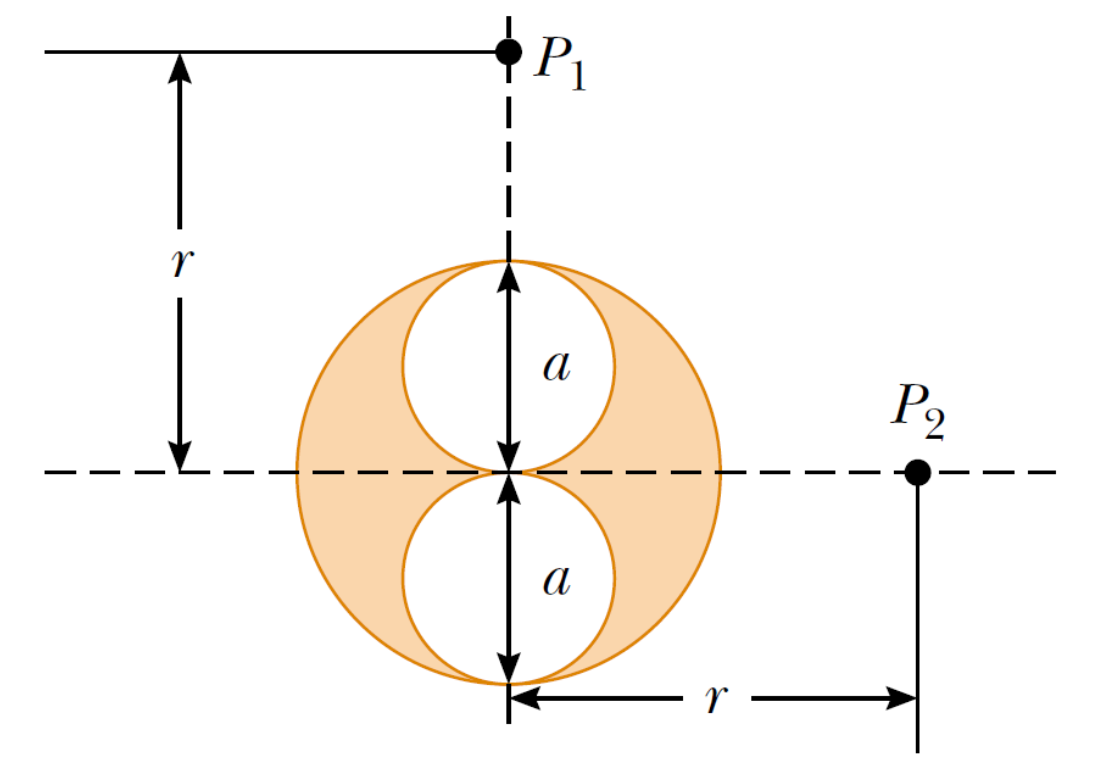
\includegraphics[scale = 0.3]{oz04/resources/Oz4Oef5.png}
\end{center}

% \begin{description}[labelwidth=1.5cm, leftmargin=!]
%     \item[Geg. :]   
%     \item[Gevr. :]  
%     \item[Opl. :]  
% \end{description}

% De oppervlakte is gelijk aan
% \begin{equation*}
%     A = \pi a^2 - 2\pi \left(\frac{a}{2}\right)^2 = \pi \frac{a^2}{2}
% \end{equation*}

\begin{description}[labelwidth=1.5cm, leftmargin=!]
    \item[Opl. :]  
    
        Neem $B_1$ het magnetisch veld door het gekleurde deel, $B_2$ het magnetisch veld door de bovenste caviteit en $B_3$ het magnetisch veld door de onderste caviteit.
        De oppervlakte $A$ waardoor stroom vloeit is
        \begin{equation*}
            A = \pi(a^2 - \frac{a^2}{2}) = \pi\frac{a^2}{2}
        \end{equation*}
        waaruit volgt dat de stroom dichtheid $J$ het volgende is
        \begin{equation*}
            J = \frac{2I}{\pi a^2}
        \end{equation*}
        m.a.w. er vloeit een stroom $2I$ door de geleider (en dus een stroom $-I$ door de caviteiten). \\
        
        \begin{enumerate}[$P_1$:]    
            \item 
                \begin{description}[labelwidth=1.5cm, leftmargin=!]
                    \item[Geg. :]  $\mu_0$, $I$, $r$, $a$
                    \item[Gevr. :] $B$ in $P_1$ ?
                    \item[Opl. :]  
                    We vinden de volgende magnetische velden
                    \begin{align*}
                        B_1 
                            &= \frac{\mu_0I}{\pi r} \\
                        B_2
                            &= \frac{\mu_0I}{2\pi\left(r - \frac{a}{2}\right)} \\
                        B_3 
                            &= \frac{\mu_0I}{2\pi\left(r - \frac{a}{2}\right)}
                    \end{align*}
                    het equivalente veld in $P_1$ is
                    \begin{align*}
                        B 
                            &= B_1 - B_2 - B_3 \\
                            &= \frac{\mu_0I}{\pi r} - \frac{\mu_0I}{2\pi\left(r - \frac{a}{2}\right)} - \frac{\mu_0I}{2\pi\left(r - \frac{a}{2}\right)} \\
                            &= \frac{\mu_0I}{\pi r}\left(\frac{2r^2-a^2}{4r^2-a^2}\right)
                    \end{align*}
                    Vectorieel:
                    \begin{equation*}
                        \Vec{B} = \frac{\mu_0I}{\pi r}\left(\frac{2r^2-a^2}{4r^2-a^2}\right) \ (-\hat{i})
                    \end{equation*}
                \end{description}    
            \item 
                \begin{description}[labelwidth=1.5cm, leftmargin=!] 
                    \item[Geg. :]  $\mu_0$, $I$, $r$, $a$
                    \item[Gevr. :] $B$ in $P_2$ ?
                    \item[Opl. :]  
                     We vinden de volgende magnetische velden
                    \begin{align*}
                        B_1 
                            &= \frac{\mu_0I}{\pi r} \\
                        B_{2,3} 
                            &=  \frac{\mu_0I}{2\pi \sqrt{r^2 + \left(\frac{a}{2}\right)^2}}
                    \end{align*}
                    waarbij $B_{2,3} = B_2 = B_3$. De horizontale componenten van $B_2$ en $B_3$ cancellen, het equivalente veld in $P_2$ is
                    \begin{align*}
                        B 
                            &= B_1 - 2B_{2,3}\cos(\theta) \\
                            &= \frac{\mu_0I}{\pi r} - \frac{\mu_0I}{\pi \sqrt{r^2 + \left(\frac{a}{2}\right)^2}}\cos(\theta) \\ 
                            &= \frac{\mu_0I}{\pi r} - \frac{\mu_0I}{\pi \sqrt{r^2 + \left(\frac{a}{2}\right)^2}} \frac{r}{\sqrt{r^2 + \left(\frac{a}{2}\right)^2}} \\ 
                            &= \frac{\mu_0I}{\pi r}\left(1 - \frac{r^2}{r^2 + \left(\frac{a}{2}\right)^2} \right) \\
                            &= \frac{\mu_0I}{\pi r}\left(\frac{2r^2+a^2}{4r^2+a^2}\right)
                    \end{align*}    
                    Vectorieel:
                    \begin{equation*}
                        \Vec{B} =\frac{\mu_0I}{\pi r}\left(\frac{2r^2+a^2}{4r^2+a^2}\right)\ (\hat{j})
                    \end{equation*}
                \end{description}
        \end{enumerate}

\end{description}
\vspace{1cm}